\chapter{Análisis del problema}

\noindent\fbox{
	\parbox{\textwidth}{
		En el capítulo se usan las herramientas para preparar el diseño del proyecto de cara a su posterior codificación.
	}
}

\section{Comparando APIs de Reconocimiento de Voz}
Como hablamos en el Capítulo 2, hoy en día existen herramientas que reconocen la voz. Algunas son de software propietario o de Software como Servicio (por ejemplo, IBM Watson SR o Google SR), pero también hay proyectos de software de código abierto que nos permiten trabajar con ello sin tener que saber los tópicos de la Inteligencia Artificial a fondo, trabajando de forma transparente al desarrollador. 

Entre estos proyectos podemos encontrar dos:
\begin{itemize}
	\item \textbf{Vosk API}:Desarrollado por Alpha Cephei en 2019 como wrapper de Kaldi , es un sistema de Reconocimiento de Voz offline que actualmente soporta 17 lenguajes y destaca por funcionar en dispositivos más limitados como la Raspberry Pi. Sus modelos más básicos son de 50 MB, pero se pueden adaptar a modelos más complejos, consiguiendo así una escalabilidad en el sistema. Además, soporta reconocimiento del habla. En su arquitectura se usa una red neuronal en conjunto con un Modelo Oculto de Markov. Usa una licencia Apache 2.0
	
	\item \textbf{Mozilla DeepSpeech}: Es una API de Reconocimiento de Voz realizado por Mozilla desde 2016, basado en un paper de Baidu sobre un sistema de Reconocimiento del Habla usando algoritmos de Deep Learning en conjunto con optimizaciones para lograr resultados más rápidos usando múltiples GPU para alimentar una Red Neuronal Recurrente que modelizara un lenguaje en base a ingentes cantidades de datos. Por tanto, acaban dando en la API una interfaz para poder usarlo en nuestros ordenadores y una serie de modelos optimizados gracias al entrenamiento que pueden realizar.
	
\end{itemize}

Para saber cuál sería la API que más nos interesara, podríamos montar un experimento donde evaluaríamos:
\begin{itemize}
	\item La facilidad de implementación
	\item La precisión de los modelos y de la API.
\end{itemize}

Este experimento se basaría en coger a varios sujetos que leyeran un mismo texto.
Esas lecturas se pasarían por un programa que emplea la API de forma que acabamos convirtiendo la voz en texto. Tras ello, se comparan ambos textos para ver el \textbf{Word Error Rate (WER)}, una métrica que mide la precisión entre lo que se ha querido decir y lo que un Reconocedor del Habla transcribe. 

El algoritmo del Word Error Rate consiste en mapear dos cadenas de texto (una indica qué se quiere decir y la otra es lo que se ha detectado) para extraer las diferencias (palabras \textbf{\textit{I}}ntroducidas, \textbf{\textit{S}}ustituidas o \textbf{\textit{R}}etiradas)  y medirlas respecto al \textbf{\textit{N}}úmero total de palabras del texto. Por tanto, su fórmula sería:

\begin{equation}
	WER = \frac{I+S+R}{N}
\end{equation}

También estaría interesante fijarnos en el CER (Character Error Rate) para ver también a nivel de caracteres qué errores se pueden encontrar en la transcripción (por ejemplo, los acentos). La fórmula sería la misma pero las inserciones, sustituciones y eliminaciones se observan letra a letra.

\begin{equation}
	CER = \frac{I_c+S_c+R_c}{N_c}
\end{equation}

Nos quedaríamos entonces con aquella implementación que sea más fácil de usar en conjunto con el modelo más preciso. 

Otra cosa que también podemos probar, de paso, es decir varios nombres propios con tal de mirar si le podemos poner nombre al Asistente, pues hoy en día es común usar como \textit{trigger word} un nombre propio (como \textit{Alexa}, \textit{Siri} o \textit{Cortana}). También podemos probar a decir acciones que debería reconocer el asistente habitualmente para funcionalidades futuras, incluso probar a decir cosas en otros idiomas (por ejemplo, canciones con títulos en inglés) para ver cómo reacciona.

Así pues, se ha redactado el siguiente texto para hacer las pruebas:

\noindent\fbox{
	\parbox{\textwidth}{
		Lúmina y Arcadia se encuentran en un portal a medio camino entre sus casas, cerca del centro comercial. Ellas habían quedado para ver la nueva película que tanto promocionaban por la tele y buscaron un momento entre sus agendas para ir a verla. 
		
		Lumi comparte uno de sus auriculares con su amiga y  enciende el móvil. Entra a Spotify y reproduce un tema de Katy Perry mientras pasean hacia su destino.
		
		Al llegar, buscan el cine y compran las entradas y las palomitas. Al entrar a la sala ven un temporizador de 5 minutos en la pantalla, que además no paraba de poner publicidad.
		
		De repente, todo se para por un corte de luz. Todo estaba a oscuras y alguien enciende la luz de su teléfono, aunque no sirve de mucho hasta que vuelve el suministro a funcionar y ya puedan ver la película.
		
		Al terminar, miran qué tiempo hace para saber si esperar a que les recojan o volver andando. Aunque lo piensan mejor tras mirar qué hora es y deciden ir a tomar un café antes de irse.
	}
}

Además de este texto tan largo, se ha probado a hacer audios más cortos, ya que suelen estar entrenados con segmentos de pocos segundos, a modo de órdenes:

\noindent\fbox{
	\parbox{\textwidth}{
		Enciende la luz.
		
		Ponme esa canción que tanto me gusta.
		
		Repite lo que diga.
		
		Para.
		
		Espera un momento.
		
		Reproduce el informativo de la mañana.
		
		Ponme una alarma a las ocho y media de la mañana.
		
		Prepara un temporizador de 5 minutos.
	}
}

De cada frase se preparará un par de variantes, ya que queremos ver cómo se comportan al nombrar varias propuestas de nombre para el producto. Estos nombres serían Arcadia y Lúmina.

En primera instancia, los cuales han grabado su voz durante la lectura. Se ha comprobado previamente de forma manual que lo que se oye es exactamente lo que se lee, ya que podría ocasionar cierto ruido el hecho de que no fuera así. Tras ello se ha tratado el audio con cada uno de los modelos y configuraciones.

En el caso de Vosk, acabaremos extrayendo su WER y CER para cada uno de los audios según su modelo oficial.

Para el caso de DeepSpeech, se ha trabajado con dos modelos ya entrenados y dos scorers, combinando ambos parámetros.

Los modelos que se probarán son:
\begin{itemize}
	\item \textbf{Polyglot}: Este modelo fue entrenado por un usuario de la Comunidad de Mozilla, entrenando un set de 812 horas con GPUs de Nvidia \cite{scribosermo}. Usa una licencia LGPL versión 3.
	\item \textbf{Rhasspy}: Este modelo estaba pensado para usarse en otro sistema de asistente de voz con una Raspberry Pi, basado en una versión anterior del modelo descrito anteriormente.
\end{itemize}

En el mismo modelo Polyglot, se nos daban dos scorers. Un scorer es un complemento del modelo del lenguaje que permite predecir qué palabra sigue. En este caso, se ha decidido usar dos para ver si causaban alguna diferencia:

\begin{itemize}
	\item \textbf{Ken}: Es un scorer ligero, con poco entrenamiento.
	\item \textbf{Poco} : Es un scorer pesado pero más completo.
\end{itemize} 

DeepSpeech también admitía dos valores extra: Alfa y Beta. Estos parámetros definen el peso del modelo del lenguaje y cuánto se penaliza por introducir una palabra. Para tener un abanico de opciones, para cada combinación se ha tratado de buscar un valor óptimo para estos parámetros, con la precisión de una décima, en un rango de 1 a 2 para el valor Alfa y un rango de 0 a 1 para el valor Beta.

Agrupamos todos los valores en esta tabla:

{\small\tabcolsep=2pt\setlength\LTleft{-35pt}	
	\begin{xltabular}{\textwidth}{|ll|l|llll|}
		\hline \multicolumn{4}{|r|}{{Continúa en la siguiente página $>>$}} \\ \hline
		\endfoot
		
		\hline
		\endlastfoot
		
		\hline
		\multicolumn{2}{|l|}{\multirow{3}{*}{}}                           & \multirow{3}{*}{\textbf{Vosk}} & \multicolumn{4}{c|}{\textbf{DeepSpeech}}                                                                                   \\ \cline{4-7} 
		\multicolumn{2}{|l|}{}                                            &                                & \multicolumn{2}{c|}{Modelo Rhasspy}                                    & \multicolumn{2}{c|}{Modelo Polyglot}              \\ \cline{4-7} 
		\multicolumn{2}{|l|}{}                                            &   
		   & \multicolumn{1}{l|}{Scorer PocoLG} & \multicolumn{1}{l|}{Scorer KenLM} & \multicolumn{1}{l|}{Scorer PocoLG} & Scorer KenLM \\ \hline
		\multicolumn{1}{|l|}{\textbf{Texto Largo}}              &         & \makecell{CER = 0,1189 \\ WER = 0,2944}  & \multicolumn{1}{l|}{\makecell{$\alpha$ = 1,2/ $\beta$ = 1 \\ CER Máx/Med: \\ 0,7787/0,8064 \\ WER Máx / Med: \\ 0,8556/0,8678 }}  & \multicolumn{1}{l|}{\makecell{$\alpha$ = 1,3/ $\beta$ = 0,8 \\ CER Máx/Med: \\ 0,7787/0,7991 \\ WER Máx / Med: \\ 0,8600/0,8760 }} & \multicolumn{1}{l|}{\makecell{$\alpha$ = 1,2/ $\beta$ = 1 \\ CER Máx/Med: \\ 0,7787/0,8065 \\ WER Máx / Med: \\ 0,8556/0,8756 }}  & \makecell{$\alpha$ = 1,3/ $\beta$ = 0,8 \\ CER Máx/Med: \\ 0,7787/0,7990 \\ WER Máx / Med: \\ 0,8400/0,8680 } \\ \hline
		\multicolumn{1}{|l|}{\multirow{2}{*}{\textbf{Frase 1}}} & Arcadia &  \makecell{CER = 0,1304 \\ WER = 0,5}  & \multicolumn{1}{l|}{\makecell{$\alpha$ = 1,6/ $\beta$ = 0.7 \\ CER Máx/Med: \\0,0000/0,0855 \\ WER Máx / Med: \\ 0,0000/0,1070 }}              & \multicolumn{1}{l|}{\makecell{$\alpha$ = 1,9/ $\beta$ = 0,9 \\ CER Máx/Med: \\ 0,0000/0,0819 \\ WER Máx / Med: \\ 0,0000/0,1690 }}             & \multicolumn{1}{l|}{\makecell{$\alpha$ = 1,6/ $\beta$ = 0,7 \\ CER Máx/Med: \\ 0,0000/0,0819 \\ WER Máx / Med: \\ 0,0000/0,1070 }}              & \makecell{$\alpha$ = 1,9/ $\beta$ = 0,9 \\ CER Máx/Med: \\ 0,0000/0,0855 \\ WER Máx / Med: \\ 0,0000/0,1690 } \\ \cline{2-7} 
		\multicolumn{1}{|l|}{}                                  & Lumina  & \makecell{CER = 0,25 \\ WER = 0,045}  & \multicolumn{1}{l|}{\makecell{$\alpha$ = 1,9 / $\beta$ = 1\\ CER Mín./Med \\0,0909/0,1292\\ WER Mín./Med \\0,25/0,285}}              & \multicolumn{1}{l|}{\makecell{$\alpha$ = 1,9/$\beta$ = 1\\ CER Mín./Med \\0,0909/0,1359\\ WER Mín./Med \\0,25/0,291}}             & \multicolumn{1}{l|}{\makecell{$\alpha$ = 1,9 / $\beta$ = 1\\ CER Mín./Med \\0,0909/0,136\\ WER Mín./Med \\0,25/0,292}}              &  \makecell{$\alpha$ = 1,9 / $\beta$ = 1\\ CER Mín./Med \\0,0909/0,129\\ WER Mín./Med \\0,25/0,29} \\ \hline
		\multicolumn{1}{|l|}{\multirow{2}{*}{\textbf{Frase 2}}} & Arcadia & \makecell{CER = 0,1136 \\ WER = 0,375}   & \multicolumn{1}{l|}{\makecell{$\alpha$ = 1/ $\beta$ =1\\ CER Mín./Med \\0,1590/0,1590\\ WER Mín./Med \\0,5/0,7118}}              & \multicolumn{1}{l|}{\makecell{$\alpha$ = 1,4/ $\beta$ =1\\ CER Mín./Med \\0,2272/0,3966\\ WER Mín./Med \\0,625/0,7138}}             & \multicolumn{1}{l|}{\makecell{$\alpha$ = 1/ $\beta$ =1\\ CER Mín./Med \\0,2272/0,396\\ WER Mín./Med \\0,625/0,7138}}              &   \makecell{$\alpha$ = 1,4/ $\beta$ =1\\ CER Mín./Med \\0,1590/0,3865\\ WER Mín./Med \\0,5/0,7118}           \\ \cline{2-7} 
		\multicolumn{1}{|l|}{}                                  & Lumina  & \makecell{CER = 0,1395 \\ WER = 0,5}  & \multicolumn{1}{l|}{\makecell{$\alpha$ = 1/ $\beta$ =1\\ CER Mín./Med \\0,1162/0,2673\\ WER Mín./Med \\0,5/0,5155}}              & \multicolumn{1}{l|}{\makecell{$\alpha$ = 1/ $\beta$ =1\\ CER Mín./Med \\0,1162/0,3046\\ WER Mín./Med \\0,5/0,6188}}             & \multicolumn{1}{l|}{\makecell{$\alpha$ = 1/ $\beta$ =1\\ CER Mín./Med \\0,1162/0,305\\ WER Mín./Med \\0,5/0,619}}              &  \makecell{$\alpha$ = 1/ $\beta$ =1\\ CER Mín./Med \\0,1162/0,2673\\ WER Mín./Med \\0,5/0,5155} \\ \hline
		\multicolumn{1}{|l|}{\multirow{2}{*}{\textbf{Frase 3}}} & Arcadia & \makecell{CER = 0 \\ WER = 0} & \multicolumn{1}{l|}{\makecell{$\alpha$ = 1,8/ $\beta$ =1\\ CER Mín./Med \\0/0,13286\\ WER Mín./Med \\0/0,183}}              & \multicolumn{1}{l|}{\makecell{$\alpha$ = 1,8/ $\beta$ =1\\ CER Mín./Med \\0/0,1077\\ WER Mín./Med \\0/0,175}}             & \multicolumn{1}{l|}{\makecell{$\alpha$ = 1,8/ $\beta$ =1\\ CER Mín./Med \\0/0,1087\\ WER Mín./Med \\0/0,177}}              &  \makecell{$\alpha$ = 1,8/ $\beta$ =1\\ CER Mín./Med \\0/0,13286\\ WER Mín./Med \\0/0,183} \\ \cline{2-7} 
		\multicolumn{1}{|l|}{}                                  & Lumina  & \makecell{CER = 0,08 \\ WER = 0,2}  & \multicolumn{1}{l|}{\makecell{$\alpha$ = 1,1/ $\beta$ =1\\ CER Mín./Med \\0,12/0,37\\ WER Mín./Med \\0,4/0,668}}              & \multicolumn{1}{l|}{\makecell{$\alpha$ = 1,1/ $\beta$ =1\\ CER Mín./Med \\0,12/0,394\\ WER Mín./Med \\0,4/0,681}}             & \multicolumn{1}{l|}{\makecell{$\alpha$ = 1,1/ $\beta$ =1\\ CER Mín./Med \\0,12/0,396\\ WER Mín./Med \\0,4/0,683}}              & \makecell{$\alpha$ = 1,1/ $\beta$ =1\\ CER Mín./Med \\0,12/0,37\\ WER Mín./Med \\0,4/0,668} \\ \hline
		\multicolumn{1}{|l|}{\multirow{2}{*}{\textbf{Frase 4}}} & Arcadia & \makecell{CER = 0,75 \\ WER = 1}  & \multicolumn{1}{l|}{\makecell{$\alpha$ = 1,8/ $\beta$ =1\\ CER Mín./Med \\0/0,132\\ WER Mín./Med \\0/0,264}}              & \multicolumn{1}{l|}{\makecell{$\alpha$ = 1,7/ $\beta$ =1\\ CER Mín./Med \\0/0,136\\ WER Mín./Med \\0/0,273}}             & \multicolumn{1}{l|}{\makecell{$\alpha$ = 1,8/ $\beta$ =1\\ CER Mín./Med \\0/0,138\\ WER Mín./Med \\0/0,275}}              &  \makecell{$\alpha$ = 1,7/ $\beta$ =1\\ CER Mín./Med \\0/0,132\\ WER Mín./Med \\0/0,264}\\ \cline{2-7} 
		\multicolumn{1}{|l|}{}                                  & Lumina  & \makecell{CER = 0,1818 \\ WER = 0,5} & \multicolumn{1}{l|}{\makecell{$\alpha$ = 1,1/ $\beta$ =1\\ CER Mín./Med \\0,1818/0,4628\\ WER Mín./Med \\0,5/0,909}}              & \multicolumn{1}{l|}{\makecell{$\alpha$ = 1,1/ $\beta$ =1\\ CER Mín./Med \\0,1818/0,4628099\\ WER Mín./Med \\0,5/0,909}}             & \multicolumn{1}{l|}{\makecell{$\alpha$ = 1,1/ $\beta$ =1\\ CER Mín./Med \\0,1818/0,46515\\ WER Mín./Med \\0,5/0,913}}              & \makecell{$\alpha$ = 1,1/ $\beta$ =1\\ CER Mín./Med \\0,1818/0,4628\\ WER Mín./Med \\0,5/0,909} \\ \hline
		\multicolumn{1}{|l|}{\multirow{2}{*}{\textbf{Frase 5}}} & Arcadia & \makecell{CER = 0 \\ WER = 0} & \multicolumn{1}{l|}{\makecell{$\alpha$ = 1,9/ $\beta$ =0,7\\ CER Mín./Med \\0,24/0,268\\ WER Mín./Med \\0,5/0,533}}              & \multicolumn{1}{l|}{\makecell{$\alpha$ = 1,9/ $\beta$ =0,6\\ CER Mín./Med \\0,24/0,296\\ WER Mín./Med \\0,5/0,579}}             & \multicolumn{1}{l|}{\makecell{$\alpha$ = 1,9/ $\beta$ =0,7\\ CER Mín./Med \\0,24/0,297\\ WER Mín./Med \\0,5/0,579}}              & \makecell{$\alpha$ = 1,9/ $\beta$ =0,6\\ CER Mín./Med \\0,24/0,268\\ WER Mín./Med \\0,5/0,533} \\ \cline{2-7} 
		\multicolumn{1}{|l|}{}                                  & Lumina  & \makecell{CER = 0,083 \\ WER = 0,25} & \multicolumn{1}{l|}{\makecell{$\alpha$ = 1,6/ $\beta$ =1\\ CER Mín./Med \\0,3333/0,4621\\ WER Mín./Med \\0,75/0,857}}              & \multicolumn{1}{l|}{\makecell{$\alpha$ = 1,6/ $\beta$ =1\\ CER Mín./Med \\0,3333/0,4676\\ WER Mín./Med \\0,75/0,862}}             & \multicolumn{1}{l|}{\makecell{$\alpha$ = 1,6/ $\beta$ =1\\ CER Mín./Med \\0,3333/0,4687\\ WER Mín./Med \\0,75/0,86}}              & \makecell{$\alpha$ = 1,6/ $\beta$ =1\\ CER Mín./Med \\0,3333/0,4621\\ WER Mín./Med \\0,75/0,857} \\ \hline
		\multicolumn{1}{|l|}{\multirow{2}{*}{\textbf{Frase 6}}} & Arcadia & \makecell{CER = 0 \\ WER = 0} & \multicolumn{1}{l|}{\makecell{$\alpha$ = 1/ $\beta$ =1\\ CER Mín./Med \\0,022/0,0909\\ WER Mín./Med \\0,14286/0,175914}}              & \multicolumn{1}{l|}{\makecell{$\alpha$ = 1,9/ $\beta$ =1\\ CER Mín./Med \\0,066/0,0989\\ WER Mín./Med \\0,1428/0,1806}}             & \multicolumn{1}{l|}{\makecell{$\alpha$ = 1/ $\beta$ =1\\ CER Mín./Med \\0,066/0,0099\\ WER Mín./Med \\0,1429/0,181}}              &\makecell{$\alpha$ = 1,9/ $\beta$ =1\\ CER Mín./Med \\0,022/0,0909\\ WER Mín./Med \\0,1428/0,1759}\\ \cline{2-7} 
		\multicolumn{1}{|l|}{}                                  & Lumina  & \makecell{CER = 0,136 \\ WER = 0,5714} & \multicolumn{1}{l|}{\makecell{$\alpha$ = 1,4/ $\beta$ =1\\ CER Mín./Med \\0,0227/0,1590\\ WER Mín./Med \\0,1428/0,3116}}              & \multicolumn{1}{l|}{\makecell{$\alpha$ = 1,4/ $\beta$ =1\\ CER Mín./Med \\0,0227/0,1641\\ WER Mín./Med \\0,1428/0,3293}}             & \multicolumn{1}{l|}{\makecell{$\alpha$ = 1,4/ $\beta$ =1\\ CER Mín./Med \\0,0227/0,165\\ WER Mín./Med \\0,1428/0,3298}}              & \makecell{$\alpha$ = 1,4/ $\beta$ =1\\ CER Mín./Med \\0,0227/0,1590\\ WER Mín./Med \\0,1428/0,31168} \\ \hline
		\multicolumn{1}{|l|}{\multirow{2}{*}{\textbf{Frase 7}}} & Arcadia & \makecell{CER = 0,1071 \\ WER = 0,1666} & \multicolumn{1}{l|}{\makecell{$\alpha$ = 1,1/ $\beta$ =0,7\\ CER Mín./Med \\0,3392/0,4589\\ WER Mín./Med \\0,67/0,761}}              & \multicolumn{1}{l|}{\makecell{$\alpha$ = 1/ $\beta$ =1\\ CER Mín./Med \\0,3392/0,4579\\ WER Mín./Med \\0,75/0,7706}}             & \multicolumn{1}{l|}{\makecell{$\alpha$ = 1,1/ $\beta$ =0,7\\ CER Mín./Med \\0,3392/0,4589\\ WER Mín./Med \\0,75/0,7715}}              & \makecell{$\alpha$ = 1/ $\beta$ =1\\ CER Mín./Med \\0,3392/0,4589\\ WER Mín./Med \\0,667/0,7610} \\ \cline{2-7} 
		\multicolumn{1}{|l|}{}                                  & Lumina  & \makecell{CER = 0,1136 \\ WER = 0,1428} & \multicolumn{1}{l|}{\makecell{$\alpha$ = 1/ $\beta$ =0,9\\ CER Mín./Med \\0,4181/0,5359\\ WER Mín./Med \\0,75/0,86845}}              & \multicolumn{1}{l|}{\makecell{$\alpha$ = 1/ $\beta$ =0,9\\ CER Mín./Med \\0,4181/0,5316\\ WER Mín./Med \\0,75/0,8622}}             & \multicolumn{1}{l|}{\makecell{$\alpha$ = 1/ $\beta$ =0,9\\ CER Mín./Med \\0,4181/0,5326\\ WER Mín./Med \\0,75/0,8632}}              &  \makecell{$\alpha$ = 1/ $\beta$ =0,9\\ CER Mín./Med \\0,4181/0,5359\\ WER Mín./Med \\0,75/0,8684}   \\ \hline
		\multicolumn{1}{|l|}{\multirow{2}{*}{\textbf{Frase 8}}} & Arcadia & \makecell{CER = 0,1272 \\ WER = 0,25} & \multicolumn{1}{l|}{\makecell{$\alpha$ = 1,4/ $\beta$ =0,8\\ CER Mín./Med \\0,1136/0,1497\\ WER Mín./Med \\0,14286/0,36953}}              & \multicolumn{1}{l|}{\makecell{$\alpha$ = 1,4/ $\beta$ =1\\ CER Mín./Med \\0,1363/0,1487\\ WER Mín./Med \\0,2857/0,3636}}             & \multicolumn{1}{l|}{\makecell{$\alpha$ = 1,4/ $\beta$ =0,8\\ CER Mín./Med \\0,1363/0,1489\\ WER Mín./Med \\0,2857/0,3643}}              & \makecell{$\alpha$ = 1,4/ $\beta$ =1\\ CER Mín./Med \\0,1136/0,1496\\ WER Mín./Med \\0,1482/0,3695} \\ \cline{2-7} 
		\multicolumn{1}{|l|}{}                                  & Lumina  & \makecell{CER = 0,2093 \\ WER = 0,4285} & \multicolumn{1}{l|}{\makecell{$\alpha$ = 1,4/ $\beta$ =0,7\\ CER Mín./Med \\0,2093/0,3096\\ WER Mín./Med \\0,4285/0,5135}}              & \multicolumn{1}{l|}{\makecell{$\alpha$ = 1,4/ $\beta$ =0,9\\ CER Mín./Med \\0,1860/0,3117\\ WER Mín./Med \\0,4285/0,5088}}             & \multicolumn{1}{l|}{\makecell{$\alpha$ = 1,4/ $\beta$ =0,7\\ CER Mín./Med \\0,1860/0,3125\\ WER Mín./Med \\0,4286/0,5095}}              &  \makecell{$\alpha$ = 1,4/ $\beta$ =0,9\\ CER Mín./Med \\0,2093/0,3096\\ WER Mín./Med \\0,4285/0,5135} \\ \hline
	\end{xltabular}
}

También se han producido gráficas con los resultados, que comentaremos a continuación:

\begin{figure}[H]
	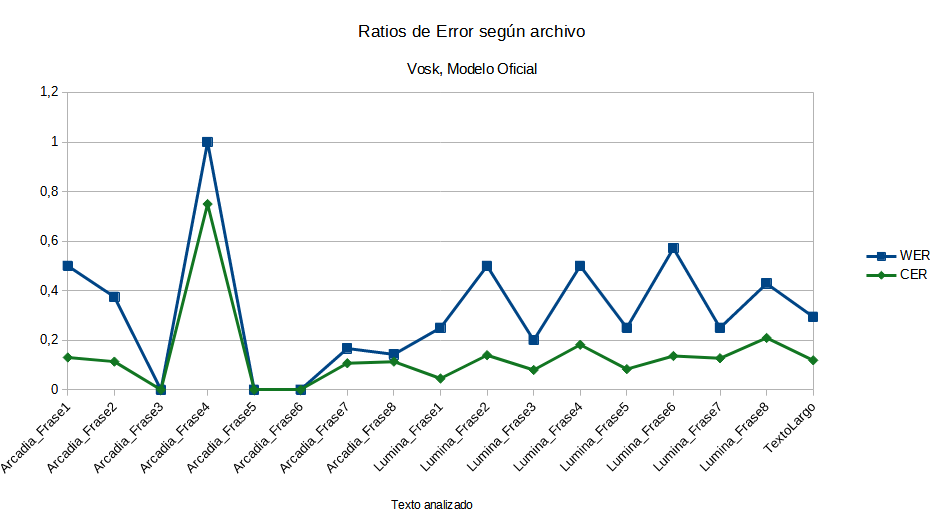
\includegraphics[width=\textwidth]{imagenes/WERCER_VoskIvan.png}
\end{figure}

\begin{table}
\begin{tabularx}{\textwidth}{|c|X|}
	\hline
	Texto & Predicción \\ \hline
	 Frase 1 (Arcadia) & arabia entiende la luz \\ \hline
	 Frase 1 (Lúmina) & lubina enciende la luz  \\ \hline
	 Frase 2 (Arcadia)& arcadia pone esa canción y tanto me gusto \\ \hline
	 Frase 2 (Lúmina)& nómina por mí esa canción que tanto me gustó \\ \hline
	 Frase 3 (Arcadia)& arcadia repite lo que diga \\ \hline
	 Frase 3 (Lúmina)& nómina repite lo que diga \\ \hline
	 Frase 4 (Arcadia)& porque había para \\ \hline
	 Frase 4 (Lúmina)& nómina para \\ \hline
	 Frase 5 (Arcadia)& arcadia espera un momento \\ \hline
	 Frase 5 (Lúmina)& nómina espera un momento \\ \hline
	 Frase 6 (Arcadia)& arcadia reproduce el informativo de la mañana \\ \hline
	 Frase 6 (Lúmina)& nómina reproducen informativos de la mañana \\ \hline
	 Frase 7 (Arcadia)& marcaría con una alarma a las ocho y media de la mañana \\ \hline
	 Frase 7 (Lúmina)& lubina con una norma a las ocho y media de la mañana \\ \hline
	 Frase 8 (Arcadia)& arcadia prepara un temporizador de cinco minutos \\ \hline
	 Frase 8 (Lúmina)& nómina preparado un temporizador de cinco minutos \\ \hline

\end{tabularx}
\end{table}

En el caso de Vosk, se aprecia que el Ratio de Error de Palabra es bastante difuso en las Frases cuando se usa Arcadia como \textit{trigger word} (de hecho, en una de las frases no ha acertado ni una palabra). Cuando vemos las frases donde se usa Lúmina como trigger word, el ratio es más alto pero menos difuso, encontrándose entre el 20 y casi el 60\%. En cuanto al texto más largo, ha captado una muy buena parte del mensaje. 
Si se tiene en cuenta que es un modelo de 55 MB una vez descomprimido, ofrece resultados bastante completos.

\begin{figure}[H]
	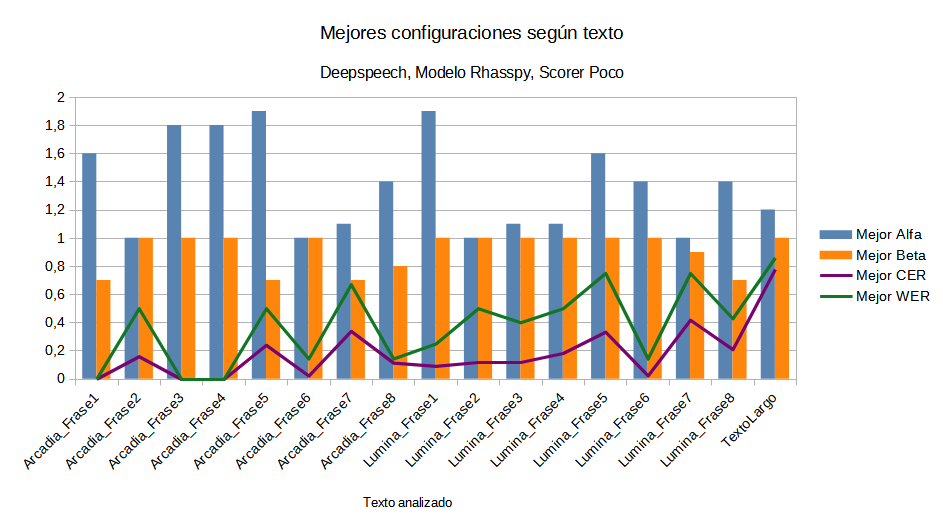
\includegraphics[width=\textwidth]{imagenes/MejoresResultados_DeepSpeechIvanPocoRhasspy.png} \\
	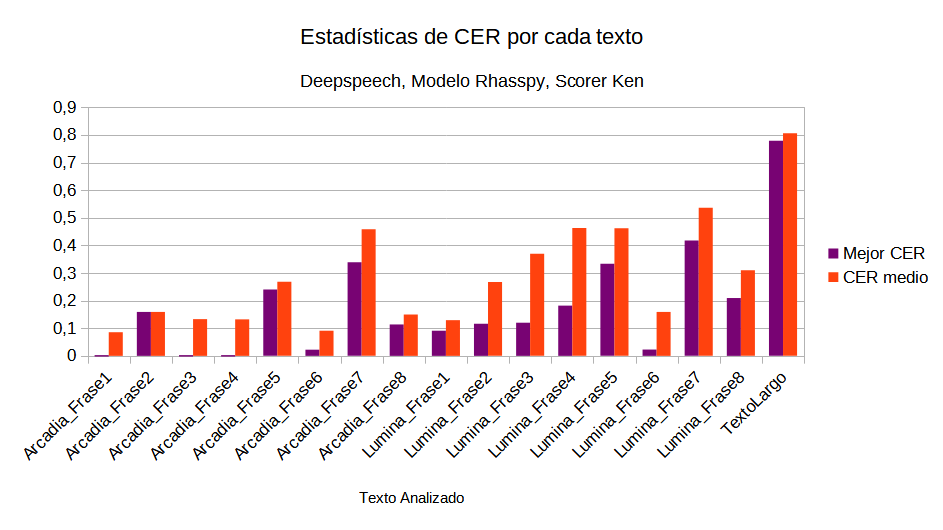
\includegraphics[width=0.5\textwidth]{imagenes/CER_DeepSpeechIvanPocoRhasspy.png} \hfill 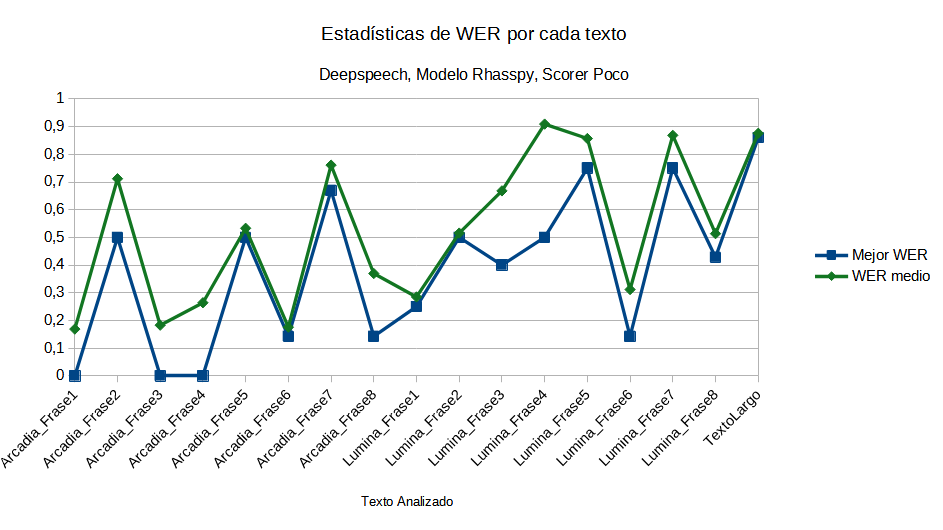
\includegraphics[width=0.5\textwidth]{imagenes/WER_DeepspeechIvanPocoRhasspy.png}
\end{figure}

Empezando en las combinaciones con DeepSpeech, donde se usa el Modelo Rhasspy y el Scorer más completo, podemos ver que los valores más óptimos de Beta se encuentran entre el 0.7 y el 1, pero los valores de Alfa son más dispares. 

Podemos apreciar también que la mayor disparidad entre lo que la red neuronal predice y lo que realmente se quería decir es del 85\% en el texto más largo. Las frases que comienzan en Arcadia parecen reconocerlas mejor que las que comienzan por Lúmina.

\begin{figure}[H]
	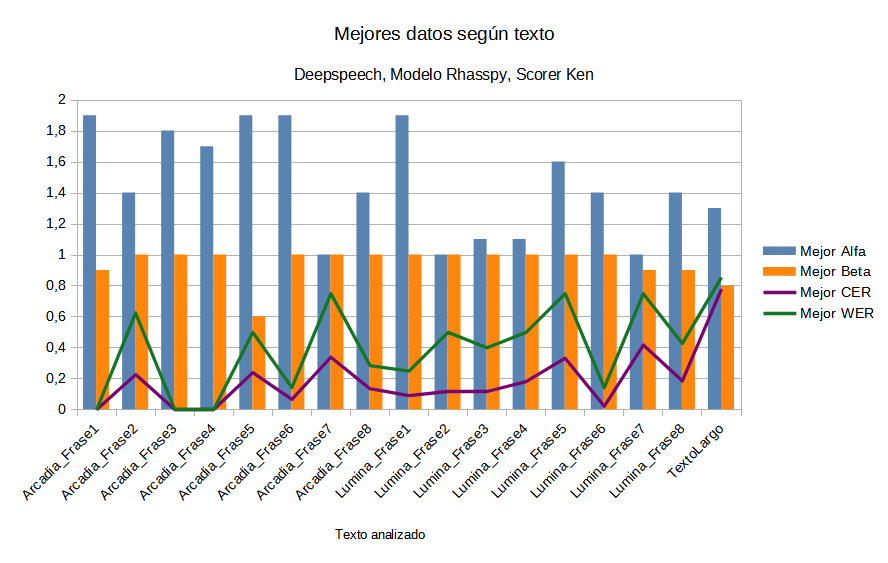
\includegraphics[width=\textwidth]{imagenes/MejoresResultados_DeepSpeechIvanKenRhasspy.png} \\
	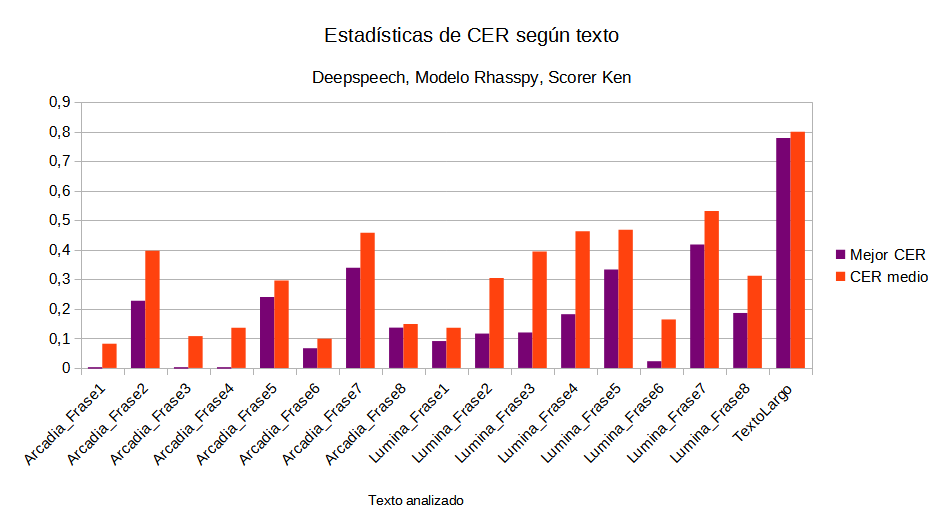
\includegraphics[width=0.5\textwidth]{imagenes/CER_DeepSpeechIvanKenRhasspy.png} \hfill 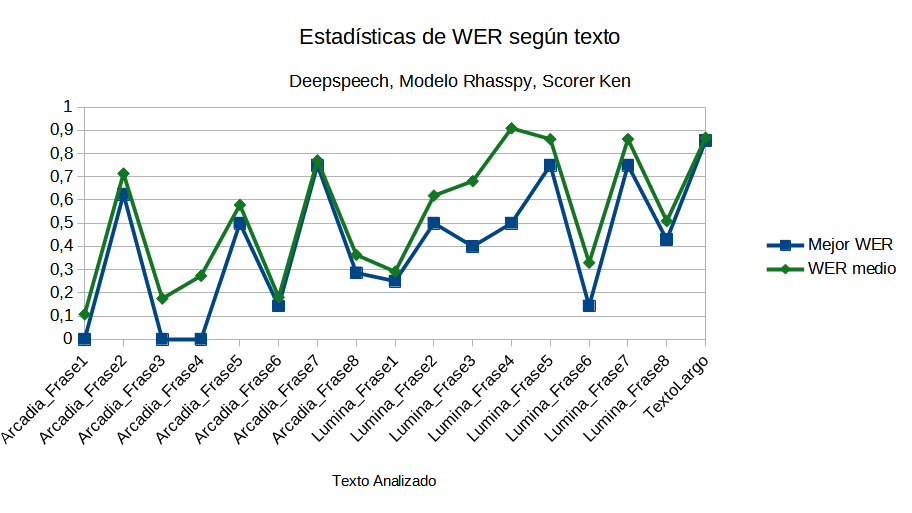
\includegraphics[width=0.5\textwidth]{imagenes/WER_DeepspeechIvanKenRhasspy.png}
\end{figure}

En esta combinación se usa el Modelo Rhasspy y el Scorer Ken, y podemos ver que los valores más óptimos de Beta se encuentran casi siempre en el 1, pero los valores de Alfa son bastante altos cuando se trata de reconocer una frase llamando a la primera opción como trigger word, generalmente entre 1,7 y 1,9. En cuanto a la segunda opción, los resultados o están muy bajos (cerca del 1,1) o altos (1,4 al 1,6 salvo la primera frase que usa un valor de 1,9).

La tónica se repite con esta combinación,donde el ratio de error en el texto largo es altísimo y reconoce muy bien el nombre de Arcadia frente al de Lúmina. En cuanto al ratio de error a nivel de caracteres, podemos ver que es muy similar al anterior.

\begin{figure}[H]
	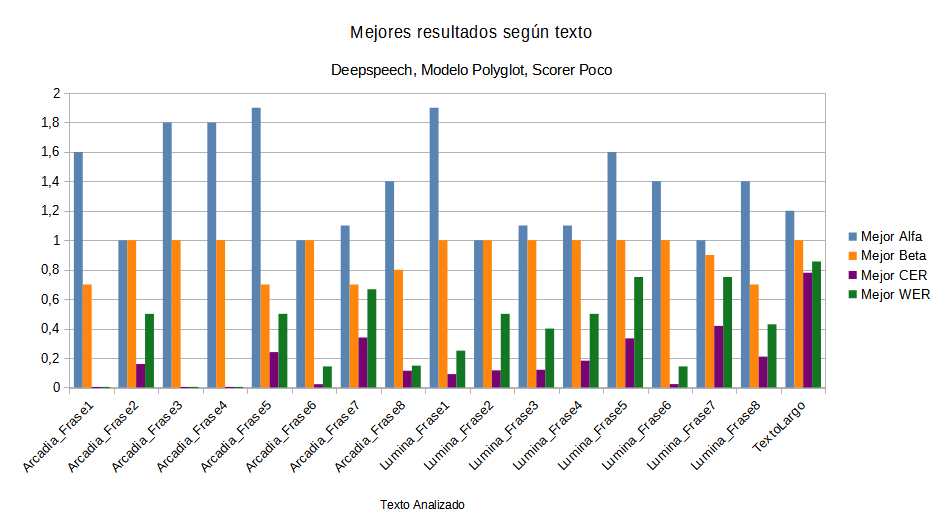
\includegraphics[width=\textwidth]{imagenes/MejoresResultados_DeepSpeechIvanPocoPolyglot.png} \\
	\includegraphics[width=0.5\textwidth]{imagenes/CER_DeepSpeechIvanPocoPolyglot.png} \hfill 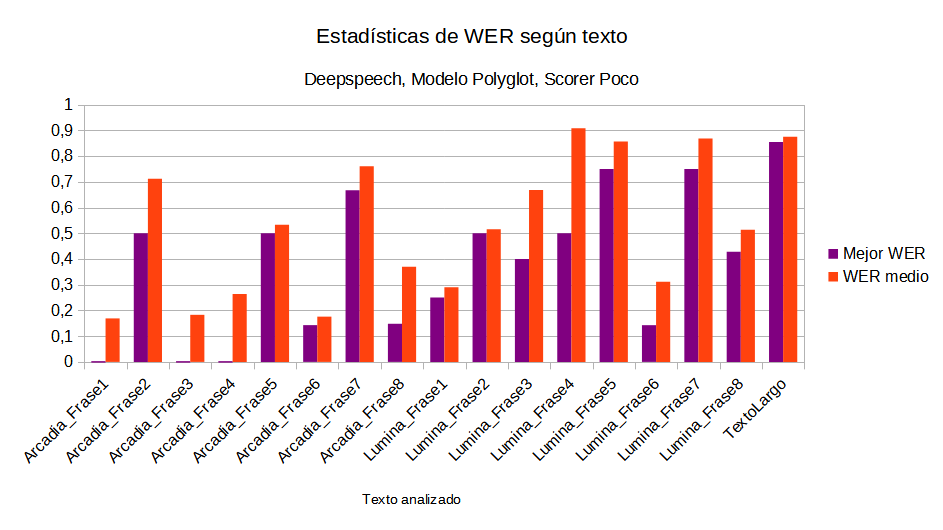
\includegraphics[width=0.5\textwidth]{imagenes/WER_DeepspeechIvanPocoPolyglot.png}
\end{figure}

En este caso se usa el modelo Polyglot con el Scorer Poco. Los valores de Beta casi siempre están a 1, o al menos más allá de 0,7. En cuanto al Alfa, hay una tendencia a valores más altos en el caso de Arcadia, y a valores más bajos en el caso de Lúmina.

El valor del WER y del CER es muy parecido a los dos anteriores. Se sigue manteniendo la tendencia de que los textos largos tienen un valor alto. De hecho, si vemos esa opción, observamos que reconoce unos cuantos segundos y encima con muchos errores.

\begin{figure}[H]
	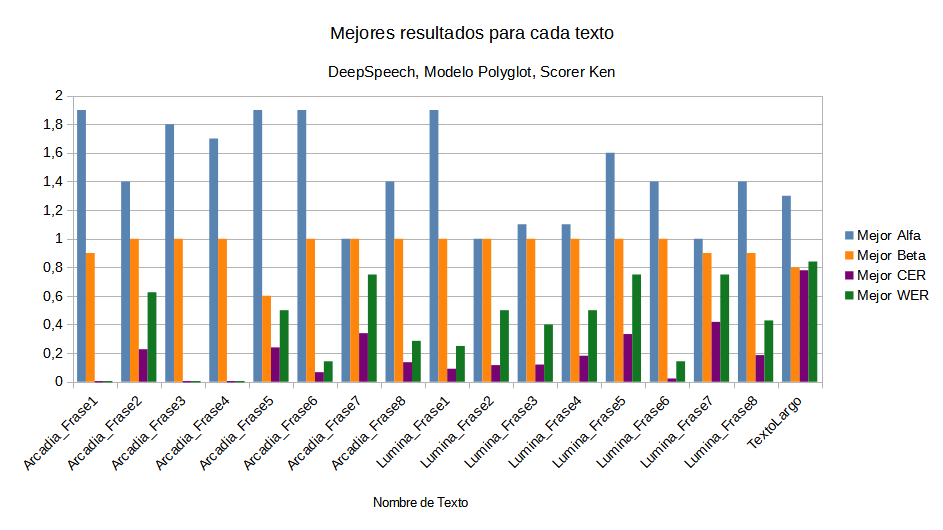
\includegraphics[width=\textwidth]{imagenes/MejoresResultados_DeepSpeechIvanKenPolyglot.png} \\
	\includegraphics[width=0.5\textwidth]{imagenes/CER_DeepSpeechIvanKenPolyglot.png} \hfill 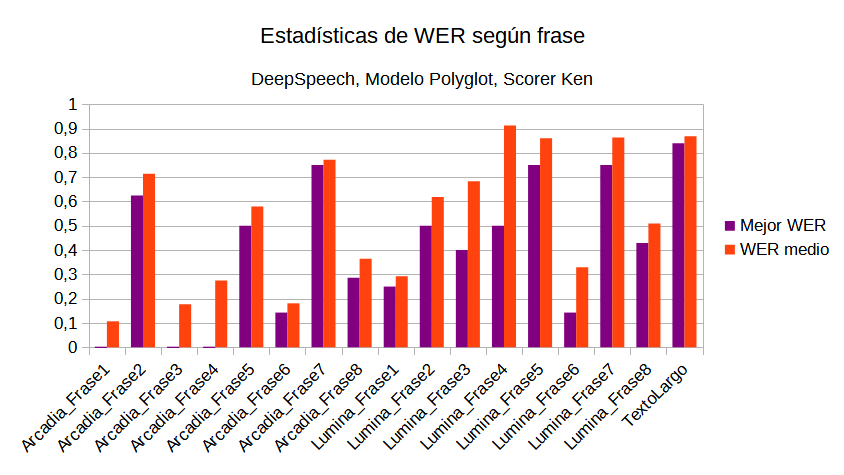
\includegraphics[width=0.5\textwidth]{imagenes/WER_DeepspeechIvanKenPolyglot.png}
\end{figure}

En la combinación del modelo Polyglot con el Scorer más liviano, los valores de Beta casi siempre están a 1, es decir, viene mejor cuanta más penalización se da por fallar. En cuanto al Alfa, hay una tendencia a valores más altos en el caso de Arcadia, y a valores más bajos en el caso de Lúmina, como en la anterior ocasión.

El valor del WER y del CER es muy parecido a los dos anteriores. Se sigue manteniendo la tendencia de que los textos largos tienen un valor alto, algo que vemos constante en los experimentos con DeepSpeech. De hecho, podemos ver en comparación lo que han deducido las 4 combinaciones de DeepSpeech y la otra API (véase tabla \ref{tab:predicts} en la página \pageref{tab:predicts})

\begin{table}
	\begin{tabularx}{\textwidth}{|c|X|}
		\hline
		\makecell{Vosk} & lo la y arcadia se encuentran en un portal a medio camino entre sus casas cerca del centro comercial ellas habían quedado para ver la nueva película que tanto proporcionaban por la tele y buscar un momento entre su agenda para ir a verla comparte un beso auriculares con su amiga y entienden entre spotify y reproduce el tema de que perdí mientras pasión hacia su destino al llegar buscar el cine y la entrada de las palomitas para la sala un temporizador de cinco minutos en la pantalla que además no paraba de poner publicidad de repente todo separa por un corte de luz toda esta oscura si alguien entiende la luz de su teléfono aunque no sirve de mucho hasta que vuelva suministro funcionar y ya puedan ver la película al terminar ya que tiempo hace para saber si esperar a que recojan o volver andando aunque lo piensa mejor tras mirar qué hora es y venir tomar un café antes de irse \\ \hline
		\makecell{DeepSpeech,\\ Modelo Rhasspy,\\ Scorer Poco} & una arcadia se encuentran en un portal a medio camino entre sus casas cerca del centro comercial ella habian quedado para ver la nueva pelicula que tanto proporcionada por la tele y buscar numenoreanos eeaaoaeecaoeee \\ \hline
		\makecell{DeepSpeech,\\ Modelo Rhasspy,\\ Scorer Ken} & una arcadia se encuentran en un portal a medio camino entre sus casas cerca del centro comercial ella habian quedado para ver la nueva pelicula que tanto proporcionada por la tele y buscar numenoreanos eeaaoaeecaoeee \\ \hline
		\makecell{DeepSpeech,\\ Modelo Polyglot,\\ Scorer Poco} & una arcadia se encuentran en un portal a medio camino entre sus casas cerca del centro comercial ella habian quedado para ver la nueva pelicula que tanto proporcionada por la tele y buscar numenoreanos eeaaoaeecaoeee \\ \hline
		\makecell{DeepSpeech,\\ Modelo Polyglot,\\ Scorer Ken} & una arcadia se encuentran en un portal a medio camino entre sus casas cerca del centro comercial ella habian quedado para ver la nueva pelicula que tanto proporcionada por la tele y buscar numenoreanos eeaaoaeecaoeee\\ \hline
		
	\end{tabularx}
	\caption{Textos que arrojan las APIs al analizar el audio más largo.}
	\label{tab:predicts}
\end{table}

Si bien hemos hablado de los datos en su propio contexto, ¿qué pasa si comparamos los resultados entre sí? Para ello se ha exportado las respuestas finales en gráficas para comparar su rendimiento ante las mismas pruebas y sacar algunas conclusiones.

\begin{figure}[H]
	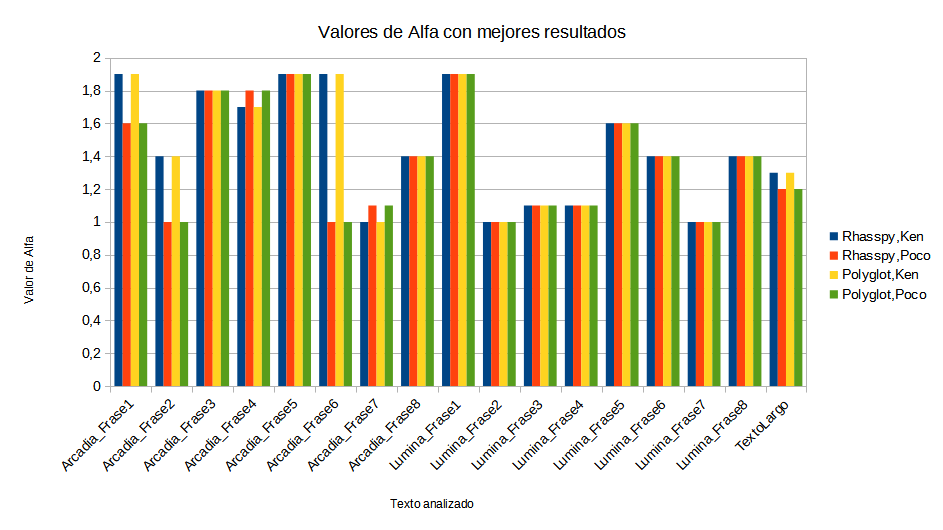
\includegraphics[width=0.5\textwidth]{imagenes/Alfas.png} \hfill 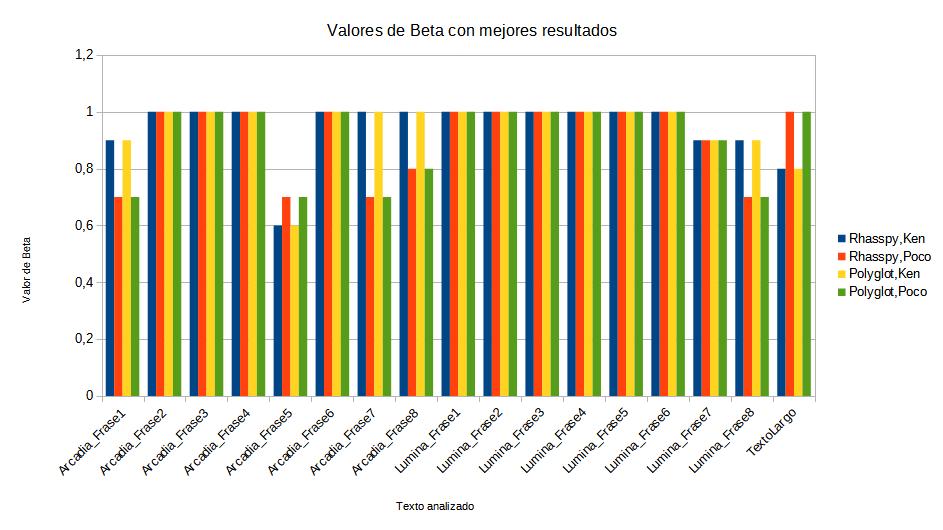
\includegraphics[width=0.5\textwidth]{imagenes/Betas.png}
\end{figure}

En el caso de DeepSpeech, los ajustes de Alfa y Beta son iguales en el caso de los modelos, por lo que usar uno u otro no nos daría ninguna ventaja. Por otro lado, los scorers sí alteran los parámetros, observando que en el Scorer Poco se da el mismo o menos peso al modelo del lenguaje en general que en Scorer Ken (como excepción podemos ver en la Frase 7 con Arcadia que el peso es menor). También se le da menos castigo en el predictor más completo (salvo en el Texto Largo y la Variante con Arcadia de la Frase 5).

\begin{figure}[H]
	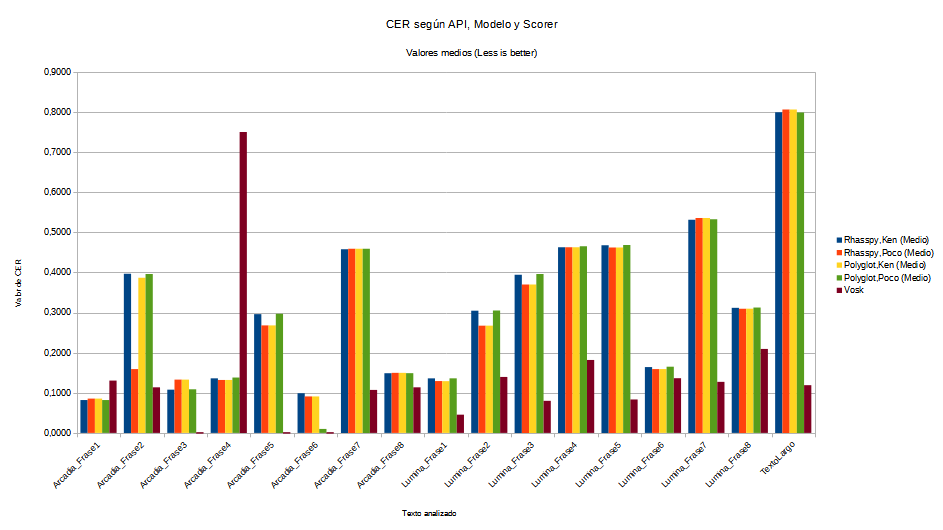
\includegraphics[width=0.5\textwidth]{imagenes/CERMedios.png} \hfill 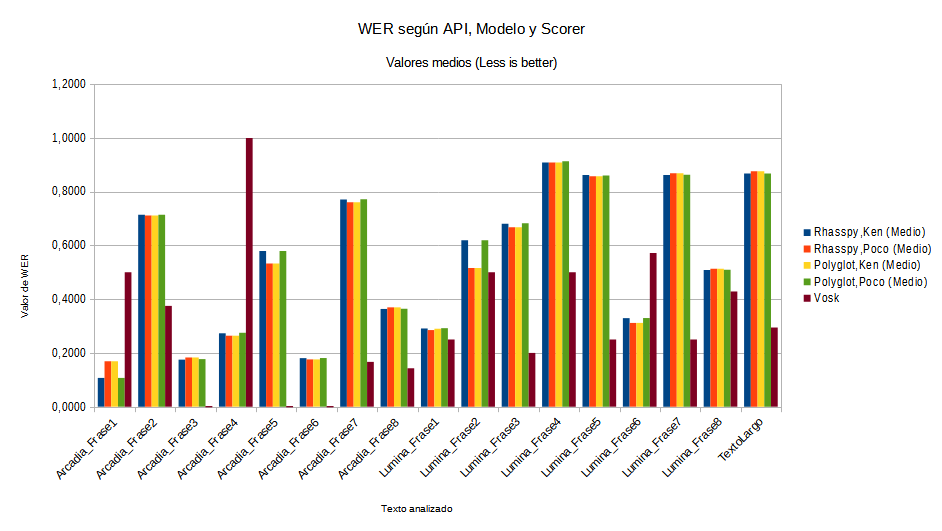
\includegraphics[width=0.5\textwidth]{imagenes/WERMedios.png}
\end{figure}

Por el Character Error Rate, vemos que al comparar letra a letra Vosk mantiene unos niveles bastante bajos salvo por su pico del 75\%. En cuanto al Ratio de Error a nivel de palabra, la cifra sube a valores de hasta un 50\% salvo en la misma frase del pico anterior, donde falla toda la predicción.
En el caso de DeepSpeech, hay muy pocas diferencias en sus valores medios entre sus 4 variantes. Como hemos visto anteriormente, debido a su comportamiento en el texto largo donde reconoce unos cuantos segundos, las relaciones de errores se disparan al tope del 80
\% en el caso del CER y del casi 90\% en el caso del WER

\begin{figure}[H]
	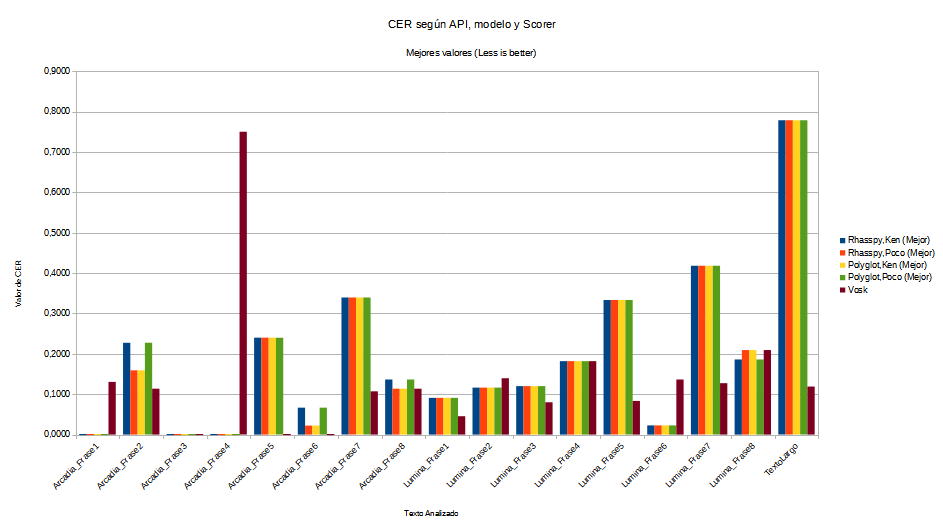
\includegraphics[width=0.5\textwidth]{imagenes/CERMejores.png} \hfill 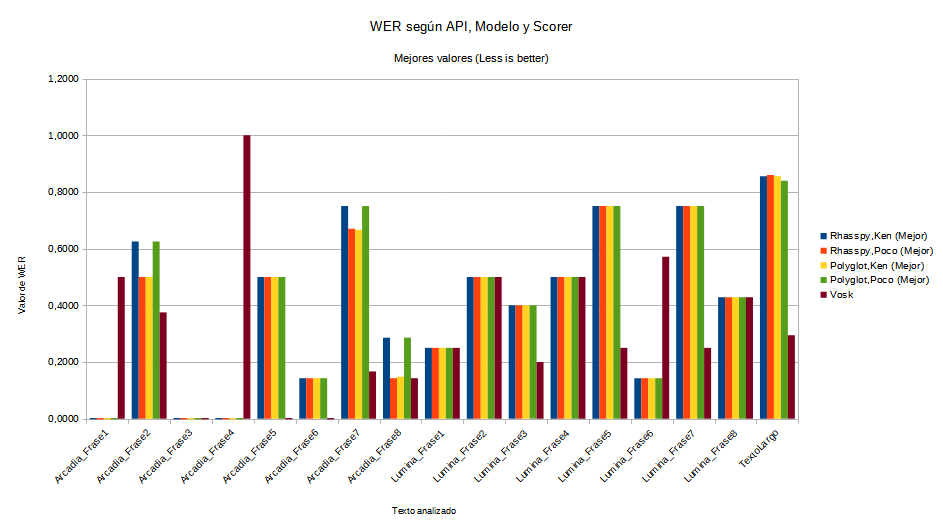
\includegraphics[width=0.5\textwidth]{imagenes/WERMejores.png}
\end{figure}

En cuanto a los resultados arrojados en las mejores generaciones, vemos que en el frente de DeepSpeech sigue siendo bastante homogéneo, si bien la combinación del Modelo Polyglot con el Scorer Ken es algo mejor en algunas ocasiones. Sin embargo, hay muchos casos donde Vosk es mejor que las 4 combinaciones, aunque podemos ver puntos aislados sorprendentes, como ver que DeepSpeech ha sido capaz de descifrar perfectamente qué se estaba hablando, cuando la alternativa falló completamente.

Otra conclusión que podemos sacar son, por ejemplo, que de los nombres propuestos, ``Arcadia'' se reconoce más veces que ``Lúmina'' (de hecho, esta última se ha reconocido sólo una vez por DeepSpeech), aunque a veces se confundan con otras palabras (como \textit{arabia}, \textit{marcaría}, o \textit{nómina}). Para permitir que se entendieran perfectamente estas palabras habría que entrenar los modelos para que las aceptaran e integraran en su vocabulario. Eso sí, hacerlo requeriría varias tarjetas gráficas y un tiempo de procesamiento de alrededor de 100 horas para hacer una sintonía fina. Otra opción sería poner alguna palabra parecida como \textit{trigger word} también, pero eso haría activarse el asistente en alguna ocasión inesperada según si la palabra es más o menos común. 

Por lo visto sobre los nombres, en este estado podemos darle nombre a nuestro Asistente en función del comportamiento de las opciones cuando se menciona esta palabra. También en este punto podemos elegir la API que menos fallo nos daría. Para ello, vamos a comprobar su promedio y desviación típica.

\begin{xltabular}{\textwidth}{|X|X|X|X|X|}
	\hline
	Método & CER Promedio & Desv. Típica de CER & WER Promedio & Desv. Típica de WER \\ \hline
	DeepSpeech + Rhasspy + Ken (Mínimo/Medio) & 0,1916/0,3115 & 0,1968/0,1966 & 0,4047/0,5349 & 0,2855/0,2763 \\ \hline
	DeepSpeech + Rhasspy + Poco (Mínimo/Medio) & 0,1850/0,2929 & 0,1993/0,1990 & 0,3845/0,5277 & 0,2814/0,2705 \\ \hline
	DeepSpeech + Polyglot + Ken (Mínimo/Medio) & 0,1850/0,3063 & 0,1993/0,1971 & 0,3844/0,5280 & 0,2805/0,2702 \\ \hline
	DeepSpeech + Polyglot + Poco (Mínimo/Medio) & 0,1916/0,3070 & 0,1968/0,2038 & 0,4038/0,5357 & 0,2840/0,2763 \\ \hline
	Vosk & 0,1375 & 0,1689 & 0,3194 & 0,2537 \\ \hline
\end{xltabular} 

Por los datos arrojados, la API que más nos convendría usar es Vosk, ya que tiende a acertar más lo que se quiere decir. 

También tenemos un nombre para nuestro asistente, pudiendo añadir algo de personalidad al producto resultante. \textit{Así que, con todos ustedes, ¡os presento a Arcadia!}

\section{Eligiendo una API de Síntesis de Voz}
Por la otra parte, sintetizar la voz nos permite ofrecer el feedback al usuario los resultados a lo que se piden. Al igual que en el Reconocimiento del Habla, las grandes compañías tienen su propia implementación en un formato "Software como servicio" (como Google TTS o IBM Watson TTS).

En este campo tenemos también otro par de APIs que usan sistemas de Código Abierto. Estos son:

\begin{itemize}
	\item \textbf{Festival TTS}: Creada por la Universidad de Edimburgo, usa una licencia del tipo X11/MIT. Se ofrece como un framework general para la síntesis de voz a través de varias APIs, ofreciendo así que se pueda usar embebido en un programa escrito en Java, dentro del propio shell o como librería de C++ (y a través de una interfaz, se puede usar con Python).
	\item \textbf{eSpeakNG}: Creado por Jonathan Duddington, se trata de un sintetizador de voz que usa el método de síntesis formante, permitiendo que las voces se representen con modelos muy ligeros, pero cuyos resultados no son muy naturales. Se licencia con GPL versión 3 \cite{gplv3}.
	Como nota aparte, se puede combinar con el sintetizador MBROLA para mejorar la voz, pero estas voces mejoradas poseen una cláusula modificada por la cual exigen que no se puede ganar beneficios con ellas en sí o embebidas en un software mayor.
	 \item \textbf{NanoTTS}: Es una reimplementación de SVOX Pico TTS, usado en la versión Open Source de Android, de la que coge las voces y la parte libre de Pico para formar un programa propio. Emplea una licencia Apache 2.0, al igual que las voces y la parte abierta.
\end{itemize}

En este ámbito, no se puede elegir el mejor programa en base a temas objetivos, sino que va más al gusto del usuario. Para ello, se ha valorado por una parte la facilidad de uso de la API, y por la otra, cómo de humana suena esa voz (de forma subjetiva).

Por la parte de facilidad de uso, he usado paquetes complementarios de pip para unir el programa con Python y así poder generar las frases desde el sistema. En ese sentido, la facilidad de uso ha sido bastante similar en el caso de \textbf{eSpeakNG} y \textbf{Festival}, ya que estas APIs requerían el uso de una librería de tratamiento de archivos .wav para hacer una copia a un archivo que tuviéramos a mano. En el caso de \textbf{NanoTTS} ha sido mucho más sencillo ya que su wrapper para Python tiene un constructor donde puedes poner cómo se llama el archivo. 

Además, en el caso del wrapper de \textbf{Festival}, hablamos de un paquete obsoleto que no deja cambiar la voz a una versión española, lo que supone un riesgo, ya que habría que parchear el código del paquete para poder cambiar la voz y otros parámetros, ya que parece estar desatendido. Por lo tanto, descartaría la opción de Festival entre los candidatos.

En cuanto a mi percepción personal sobre cómo suenan las otras dos voces:
\begin{itemize}
	\item En el caso de \textbf{eSpeak}, no se nota muy robótica y además se puede personalizar bastante, pero hay algo en el producto generado que falla, y es que sale una especie de fonema extraño que suena en cada palabra, lo que puede ser algo molesto.
	\item Sobre \textbf{NanoTTS}, me ha parecido una voz más realista con ajustes bastante similares a los del anterior, siendo su pega más relevante unas pausas quizás un poco más largas de lo normal.
\end{itemize}

En conclusión, usaré NanoTTS para que Arcadia nos hable. Pero ahora que nos puede hablar y escuchar, sólo nos quedaría conectar ambas partes.

\section{Relacionando preguntas y respuestas.}
Una vez que podamos pasar a texto las preguntas y que además el texto que respondamos se pueda convertir a voz, falta dotar a nuestro Asistente con algo de funcionalidad y una base de conocimientos para que nos pueda decir algo coherente.

En este caso, nos encontramos con algunas alternativas que responden a distintos tipos de funcionamiento:

\begin{itemize}
	\item \textbf{Pattern-matching}
	Aquí nos podemos encontrar algunos casos como:
	\begin{itemize}
		\item \textbf{AIML} Ya he estado familiarizado con este lenguaje de marcado anteriormente, en la asignatura de Inteligencia Artificial. Si bien permitía hacer cierta funcionalidad, no puede usar peticiones de APIs para poder completar información en sus últimas versiones, por lo que queda descartada. Además, su sintaxis puede llegar a ser compleja de entender, ya que se necesita una estructura con muchas etiquetas para funciones más dificultosas.
		\item \textbf{RiveScript} Es una versión un poco menos liosa de AIML, pero tiene mucha de su funcionalidad, aparte de algunas funciones extra (como más condicionales o temas que puedan ser heredados de otros temas de conversación). Sin embargo, hacer un embed de Python con un cliente de RiveScript conllevaría un tiempo considerable.
		\item \textbf{ChatScript} En este caso hablamos de un lenguaje de script superior a los anteriores, pero cae en el mismo problema que RiveScript. Y es que su único cliente está desarrollado en C, si bien se podría adaptar a Python gracias a la librería que tiene para invocar funciones de C.
	\end{itemize}	
	\item \textbf{Procesamiento del lenguaje natural (NLP)}
	Si bien hay opciones propietarias como \textbf{\underline{DialogFlow}}, al mirar opciones de Código Abierto me costó dar con uno, pero finalmente apareció la opción de usar \textbf{\underline{Rasa}}, que aunque no tenía mucha documentación en español, era bastante completa y esmerada, y con bastantes vídeos y tutoriales que me ayudaron a entender cómo usarlo.
\end{itemize}

Al comparar ChatScript y Rasa para decidir cuál usar, observé que el hecho de que Rasa esté en continuo desarrollo, la flexibilidad de sus modelos y la facilidad para entrenarlos me ha servido de punto de inflexión para elgir esta herramienta frente a la opción por patrones.
	
\section{Diseñando el problema}

En resumen hasta ahora, hemos conseguido los tres grandes ingredientes que componen a nuestro proyecto. Ahora que los tenemos, ya nos queda preparar el problema y sus diagramas para facilitar el desarrollo.

\subsection{Diagrama de casos de uso}
En este proyecto, los casos de uso en general tienen sólo un actor humano, que sería el usuario que interactúa con el software. Pero también hemos de incluir un actor que intervendría en el desarrollo, que en este caso sería el chatbot, ya que si bien se desarrolla, al final interactúa con el software y sería capaz de funcionar independientemente.

El flujo básico de Arcadia estaría definido por el siguiente diagrama de casos de uso, donde ambos actores interactúan en el transcurso entre que el usuario diga una petición y el mismo reciba la respuesta.

\begin{figure}[H]
	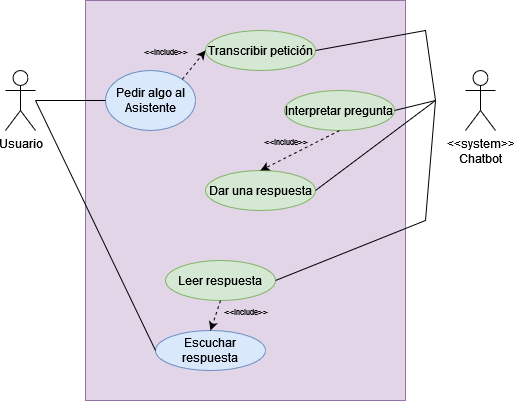
\includegraphics[width=\textwidth]{imagenes/DiagramaCasosUso.png}
	\caption{Diagrama de casos de uso.}
\end{figure}

\subsection{Diagrama de clases}
\subsubsection{Grabación y streaming de audio}
Para la grabación del audio podemos usar FFmpeg o PyAudio indistintamente, ya que ambos sistemas de codificación del audio son bastante capaces para esta tarea. Claro, esto implicaría hacer uso del patrón Adaptador para crear una abstracción entre los métodos o ejecuciones del software existente y nuestro sistema para cada opción.
En este caso podríamos seguir esta manera de construir software para tener varias versiones de esa funcionalidad con sistemas distintos. (Aunque en la práctica lo más probable es que lo haga con uno de ellos, pero gracias a ello podemos darle modularidad al sistema para cambiarlo en cualquier momento).

\begin{figure}[H]
	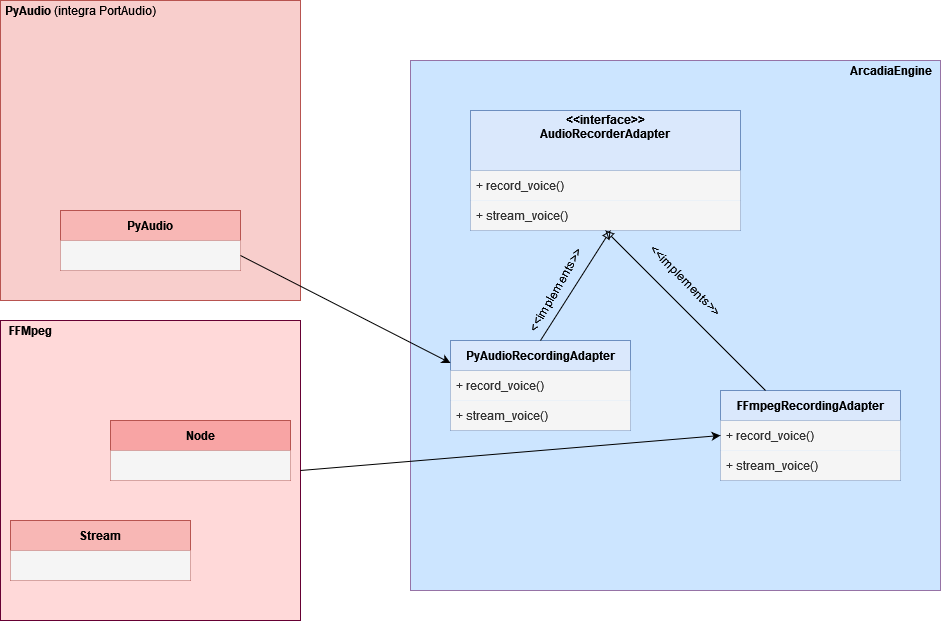
\includegraphics[width=\textwidth]{imagenes/DiagramaClases_Grabacion.png}
	\caption{Diagrama de clases relacionadas con la grabación del sonido.}
\end{figure}

\subsubsection{Reconocimiento de voz}
Para el reconocimiento de voz se hará uso de una clase que sirva de interfaz a las APIs que lo requieran, las cuales tendrán para poder usarse en el resto de la implementación una clase que sirva de adaptador. De esta manera, si quisiéramos usar otra API, sólo tendríamos que implementar los métodos del adaptador.
\begin{figure}[H]
	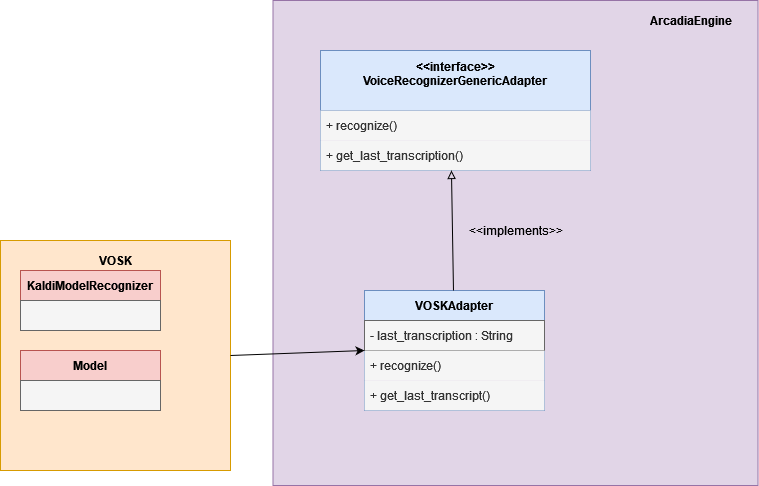
\includegraphics[width=\textwidth]{imagenes/DiagramaClases_SR.png}
	\caption{Diagrama de clases relacionadas con el Reconocimiento del habla.}
\end{figure}
\subsubsection{Procesamiento de la petición y creación de una respuesta}
Para procesar la petición, usaremos un adaptador como antes. En nuestro caso, además, trataremos con peticiones HTTP a través de REST entre nuestra implementación y Rasa, ya que se aloja en un puerto de nuestro PC escuchando las peticiones.

En la parte de Rasa, según su documentación, para desarrollar funcionalidades más complejas, podemos implementar en su entorno, en un fichero Python, clases que heredan de Action. Al estar alojados en otro puerto donde se comunica principalmente con el puerto de Rasa, interactúan entre sí para dar la respuesta.

Aquí podemos ver un detalle de las clases y sus relaciones, en este sentido:
\begin{figure}[H]
	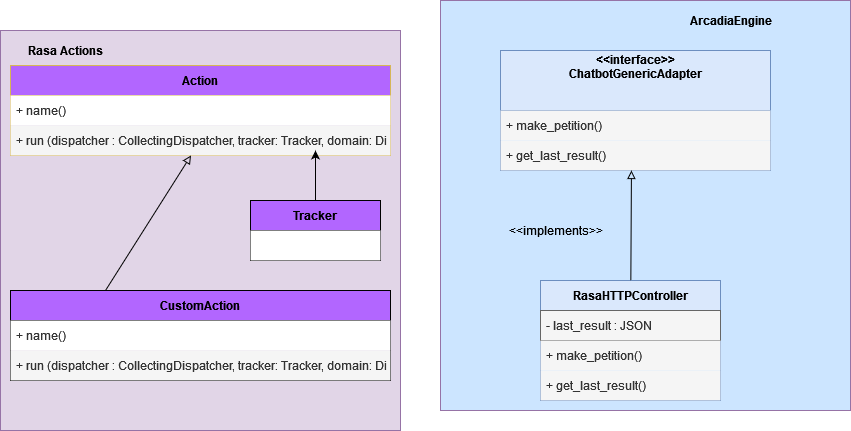
\includegraphics[width=\textwidth]{imagenes/DiagramaClases_Chatbot.png}
	\caption{Diagrama de clases relacionadas con la interacción con el Chatbot.}
\end{figure}
\subsubsection{Síntesis de voz}
De forma análoga al reconocimiento de voz, la síntesis precisará de un adaptador para facilitar el funcionamiento interno del asistente. De esta manera, lo conectaremos a NanoTTS para que nos convierta el texto a Voz.

\begin{figure}[H]
	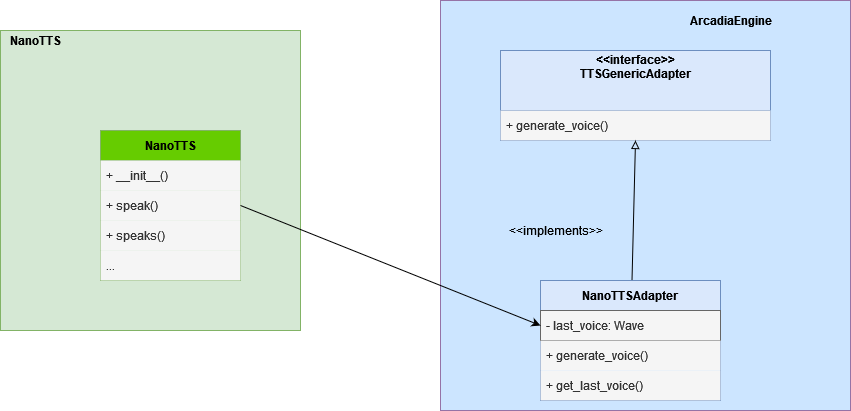
\includegraphics[width=\textwidth]{imagenes/DiagramaClases_TTS.png}
	\caption{Diagrama de clases relacionadas con la Síntesis de Voz.}
\end{figure}
\subsubsection{Reproducción de las respuestas}
Para la reproducción del audio podemos usar de nuevo FFmpeg o PyAudio indistintamente, ya que ambos sistemas pueden grabar y reproducir audio . Ya que esán importados, habría que hacer otros adaptadores sólo para el sentido de la reproducción.

\begin{figure}[H]
	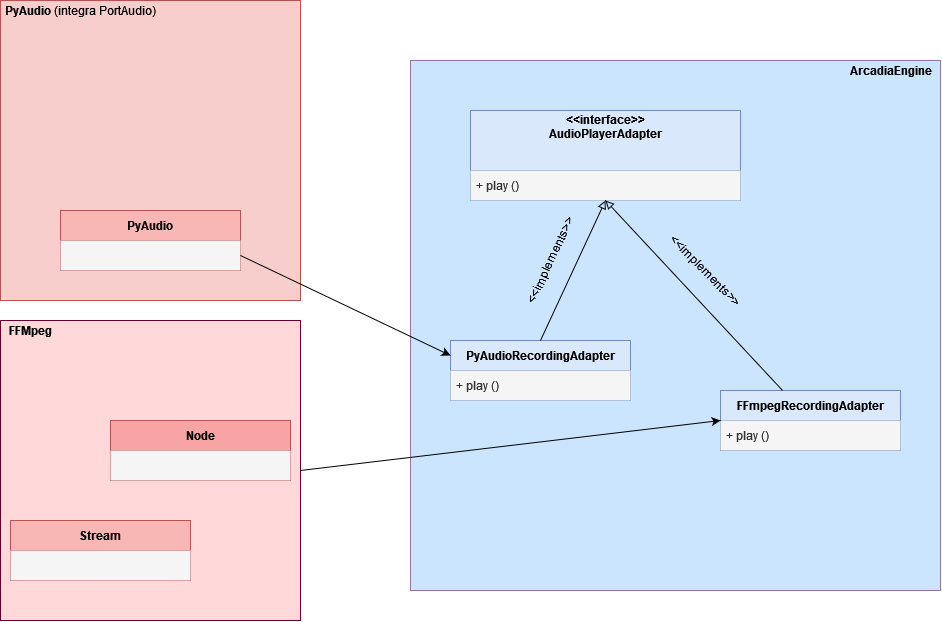
\includegraphics[width=\textwidth]{imagenes/DiagramaClases_Reproduccion.png}
	\caption{Diagrama de clases relacionadas con la reproducción del sonido.}
\end{figure}

El resultado final del diagrama de clases está en la página ... .
\begin{landscape}
	\begin{figure}
		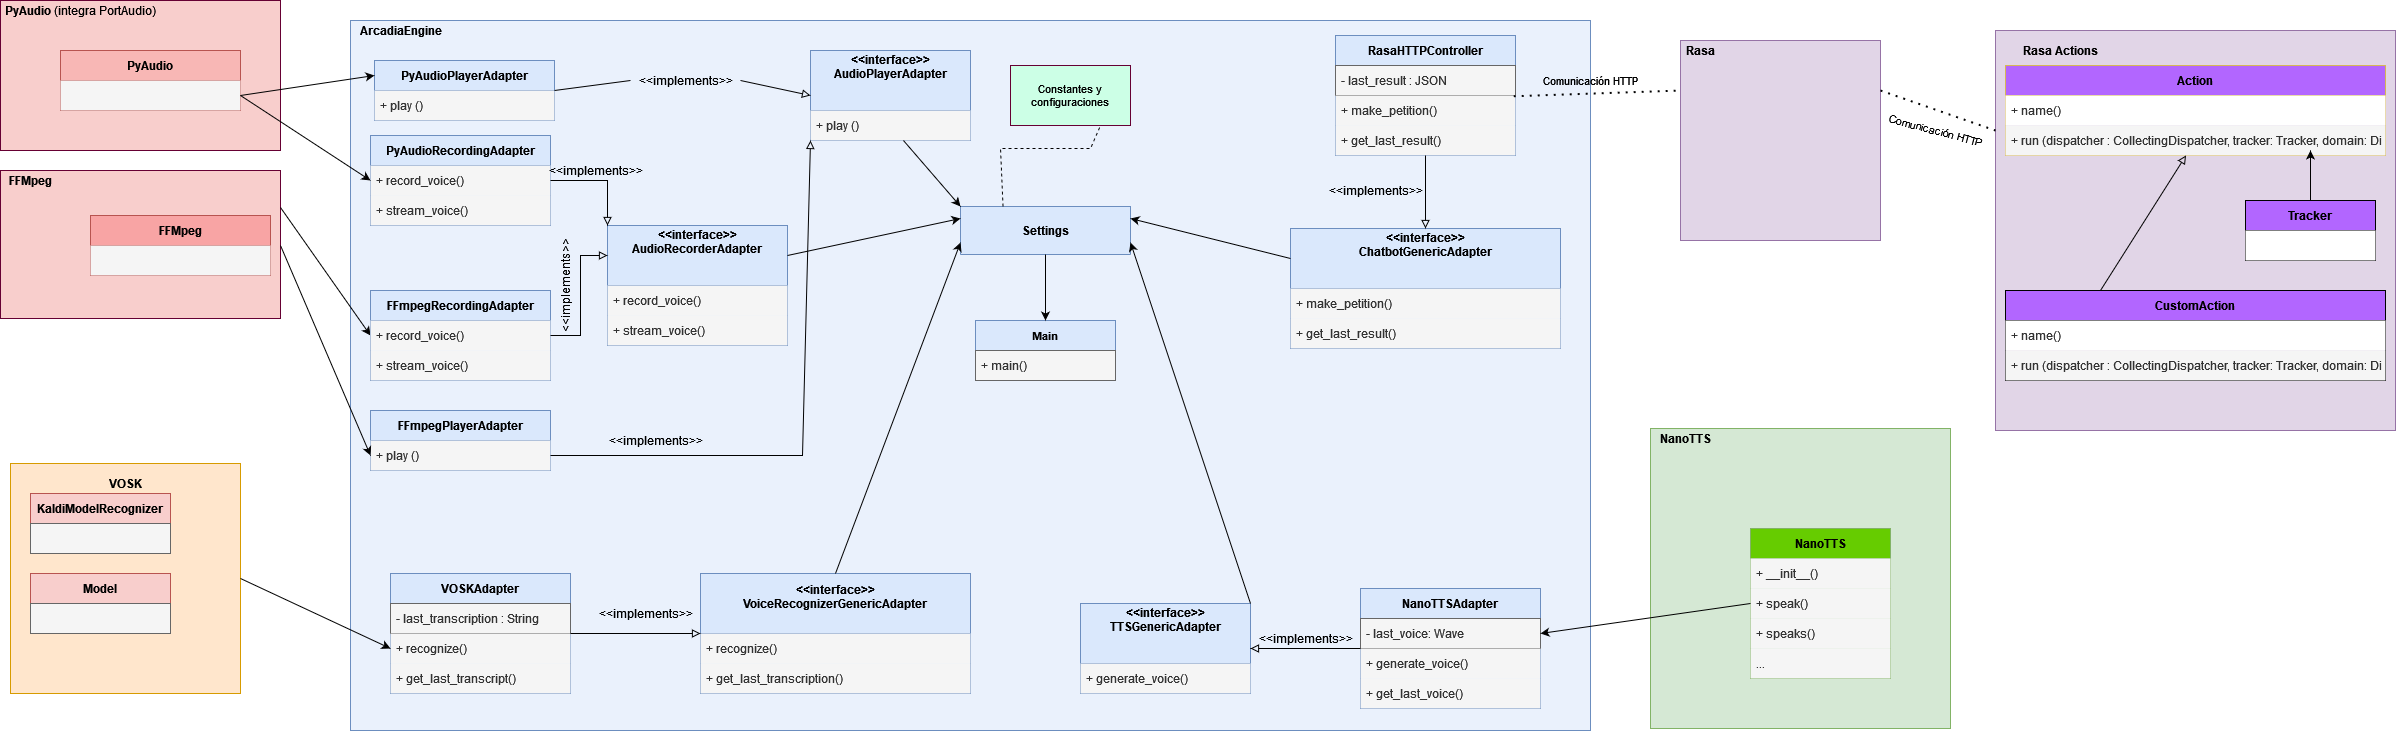
\includegraphics[width=1.5\textwidth]{imagenes/DiagramaClases_General.png}
		\caption{Diagrama de clases general.}
	\end{figure}
\end{landscape}
\subsection{Diagrama arquitectónico}
Por lo que vemos, nos encontramos con una arquitectura que dispone de programas externos que podemos usar en nuestro software gracias a sus respectivas APIs. Por nuestra parte, primero adaptamos toda su funcionalidad a nuestro ámbito en una serie de adaptadores para simplificar la información que luego llegará o saldrá de nuestro núcleo, que define el flujo básico del proyecto.

Por otra parte, tenemos una comunicación con Rasa, que a su vez tiene otra comunicación con Rasa Actions, para atender las peticiones más complejas. Desde Rasa Actions también se hará la gestión de consultas a algunas páginas de Internet.

Por tanto, nos quedaríamos con la siguiente arquitectura:

\begin{figure}[H]
	\includegraphics[width=\textwidth]{imagenes/DiagramaArquitectónico.png}
	\caption{Diagrama de la arquitectura de Arcadia.}
\end{figure}

\subsection{Diagrama de flujo general}
 
